E' stata implementata la macro \textit{AnaBragg.C} per misurare la larghezza temporale dei segnali. Sono stati presi come riferimenti temporali i valori per i quali il segnale
passa per il 40 \% del valore massimo. 
Dalle misure a 400 mb è stata ricavata la velocità di drift. A causa della bassa pressione infatti, le particelle alfa hanno un range sufficiente ad arrivare alla fine della camera. La loro curva è perciò limitata in range temporale. 
Utilizzando la misura della larghezza temporale dei segnali a 400 $mb$ è stata calcolata la velocità di drift, 
tramite la formula per il calcolo della velocità:

$$ v=\frac{lunghezza\;camera}{range\; temporale} $$

La lunghezza della camera di Bragg è stata considerata $120 \pm 1$ mm.

\begin{tabella}
 \centering
 
\begin{center}
\begin{tabulary}{\textwidth}{CCC}
\toprule
 p($mb$)& range $\pm$ $\sigma_{range}$ ($mm$) &  width $\pm$ $\sigma_{width}$($\mu$ s)\\
400&	113.3$\pm$	0.7&	69.52$\pm$	0.04\\
450&	103.2$\pm$	0.6&	63.33$\pm$	0.04\\
500&	94.0$\pm$	0.6&	57.67$\pm$	0.04\\
550&	84.6$\pm$	0.5&	51.93$\pm$	0.03\\
600&	72.5$\pm$	0.4&	44.46$\pm$	0.02\\
650&	66.9$\pm$	0.4&	41.06$\pm$	0.05\\
\bottomrule
\end{tabulary}
\end{center}



 
 \caption{Tabella range spaziali e width temporali primo picco}
 \label{tab:range_picco1.tex}
\end{tabella}

\begin{tabella}
 \centering
 
\begin{center}
\begin{tabulary}{\textwidth}{CCC}
\toprule

 p($mb$)& range $\pm$ $\sigma_{range}$ ($mm$) &  width $\pm$ $\sigma_{width}$($\mu$ s)\\
400&	124.0$\pm$  0.8&	76.05$\pm$	0.06\\
450&	111.8$\pm$	0.7&	68.56$\pm$	0.05\\
500&	102.2$\pm$	0.6&	62.68$\pm$	0.05\\
550&	91.7$\pm$	0.6&	56.28$\pm$	0.03\\
600&	78.3$\pm$	0.5&	48.02$\pm$	0.03\\



 \bottomrule
\end{tabulary}
\end{center}
 
 \caption{Tabella range spaziali e width temporali secondo picco}
 \label{tab:range_picco2.tex}
\end{tabella}

\begin{tabella}
 \centering
 
\begin{center}
\begin{tabulary}{\textwidth}{CCC}
\toprule
p($mb$)& range $\pm$ $\sigma_{range}$ ($mm$) &  width $\pm$ $\sigma_{width}$($\mu$ s)\\
450&	119.6$\pm$	0.7&	73.37$\pm$	0.05\\
500&	109.8$\pm$	0.8&	67.35$\pm$	0.05\\
550&	98.7$\pm$	0.7&	60.56$\pm$	0.05\\
600&	84.0$\pm$	0.6&	51.56$\pm$	0.04\\
\bottomrule
\end{tabulary}
\end{center}
 
 \caption{Tabella range spaziali e width temporali terzo picco}
 \label{tab:range_picco3.tex}
\end{tabella}



\begin{grafico}
 \centering
 \resizebox{\textwidth}{!}{%
 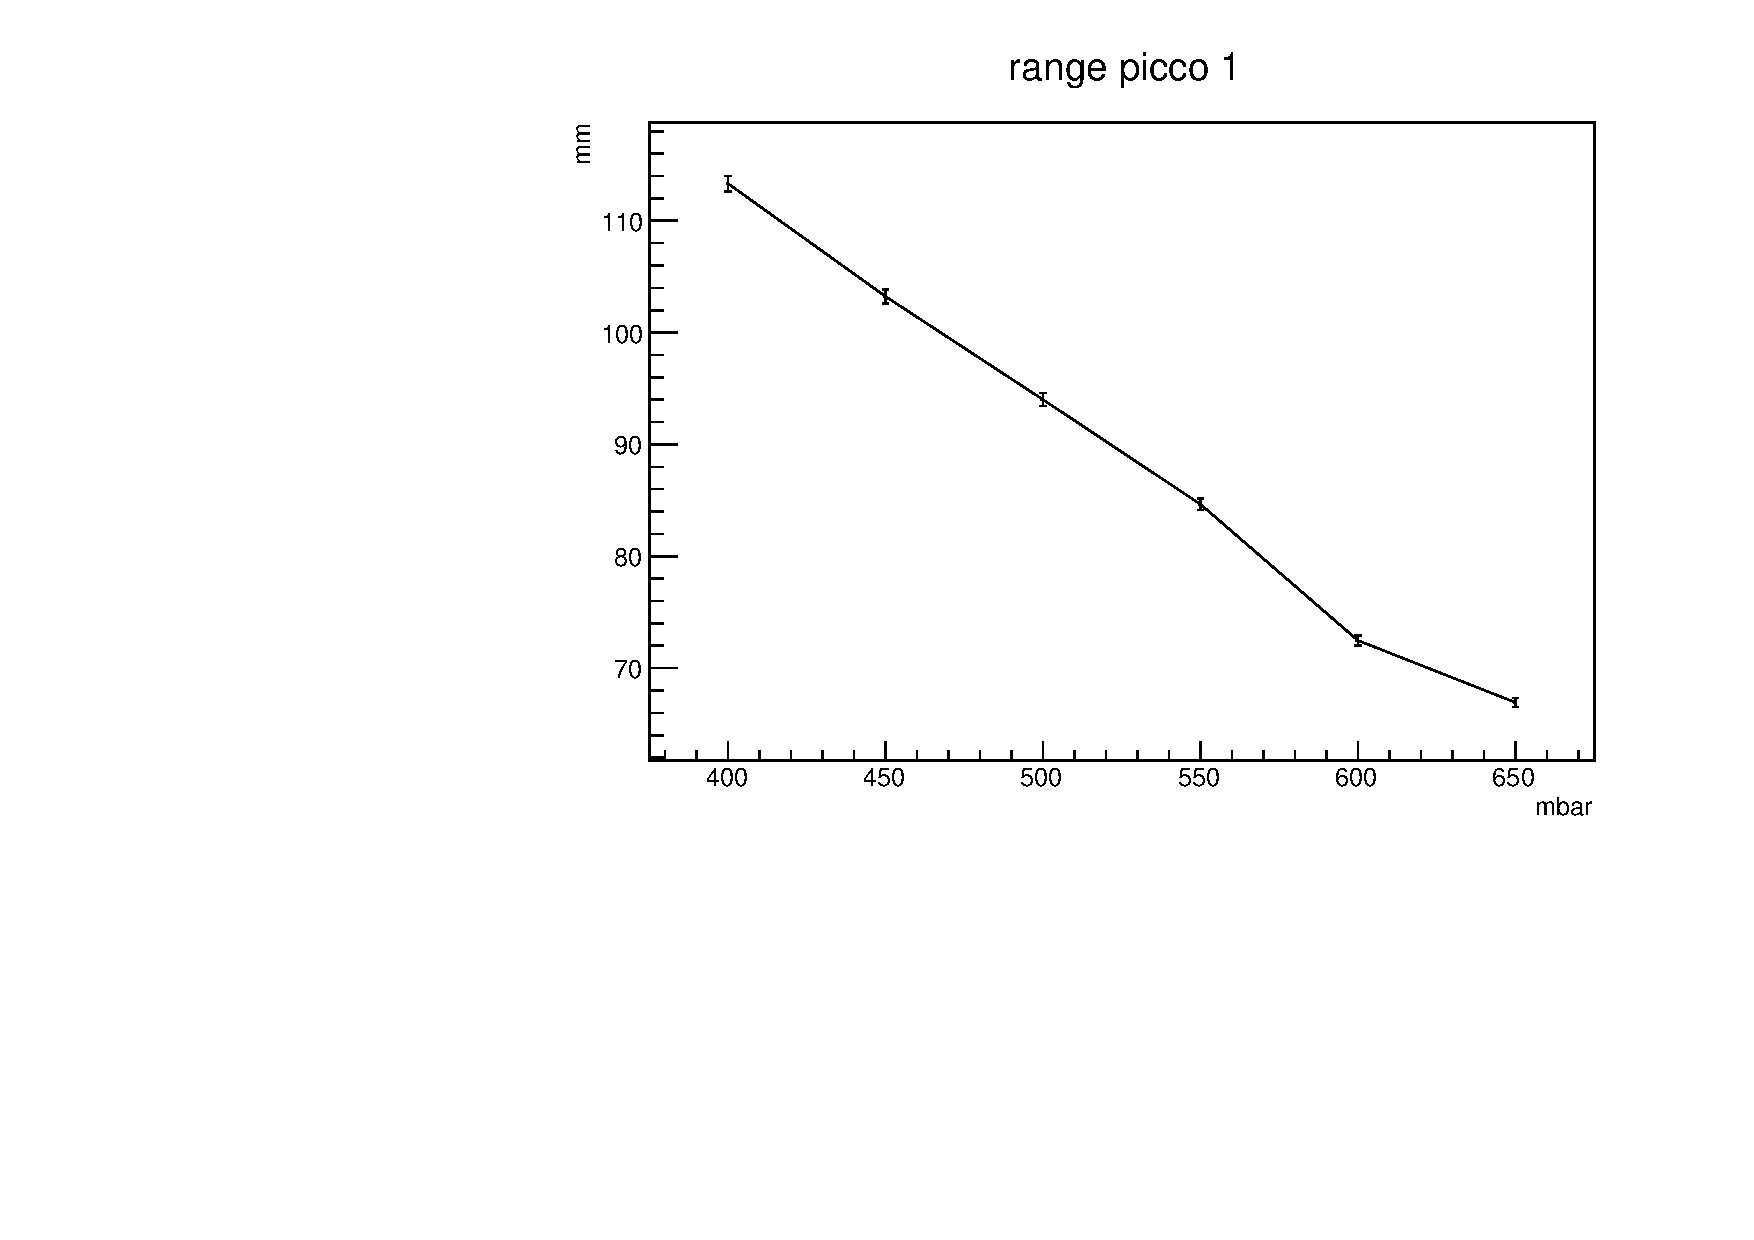
\includegraphics{../grafici/risultati/rangepicco1.pdf}
 }%
 \caption{Grafico Range ($mm$) su Pressione ($mb$) picco 1} 
 \label{gr:rangepicco1.tex} 
\end{grafico}


\begin{grafico}
 \centering
 \resizebox{\textwidth}{!}{%
 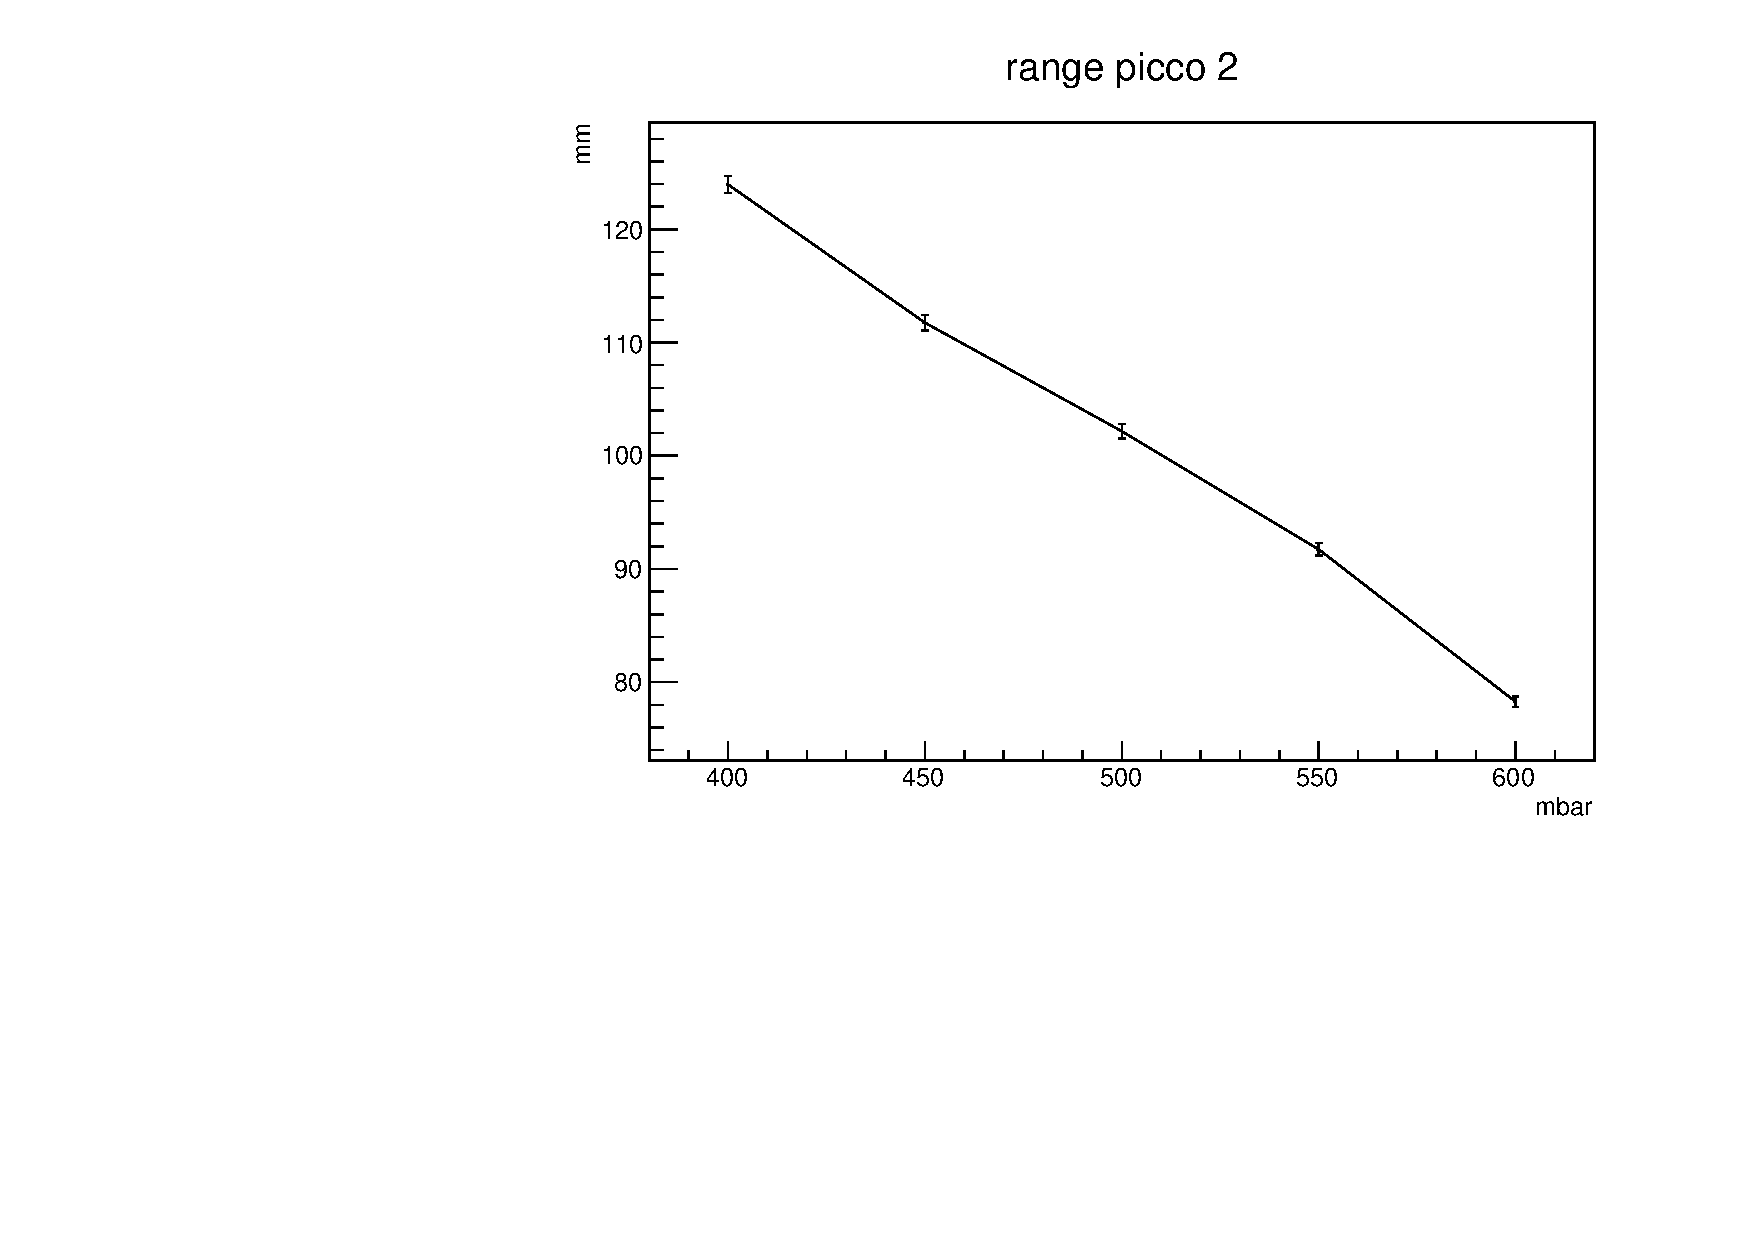
\includegraphics{../grafici/risultati/rangepicco2.pdf}
 }%
 \caption{Grafico Range ($mm$) su Pressione ($mb$) picco 2} 
 \label{gr:rangepicco2.tex} 
\end{grafico}

\begin{grafico}
 \centering
 \resizebox{\textwidth}{!}{%
 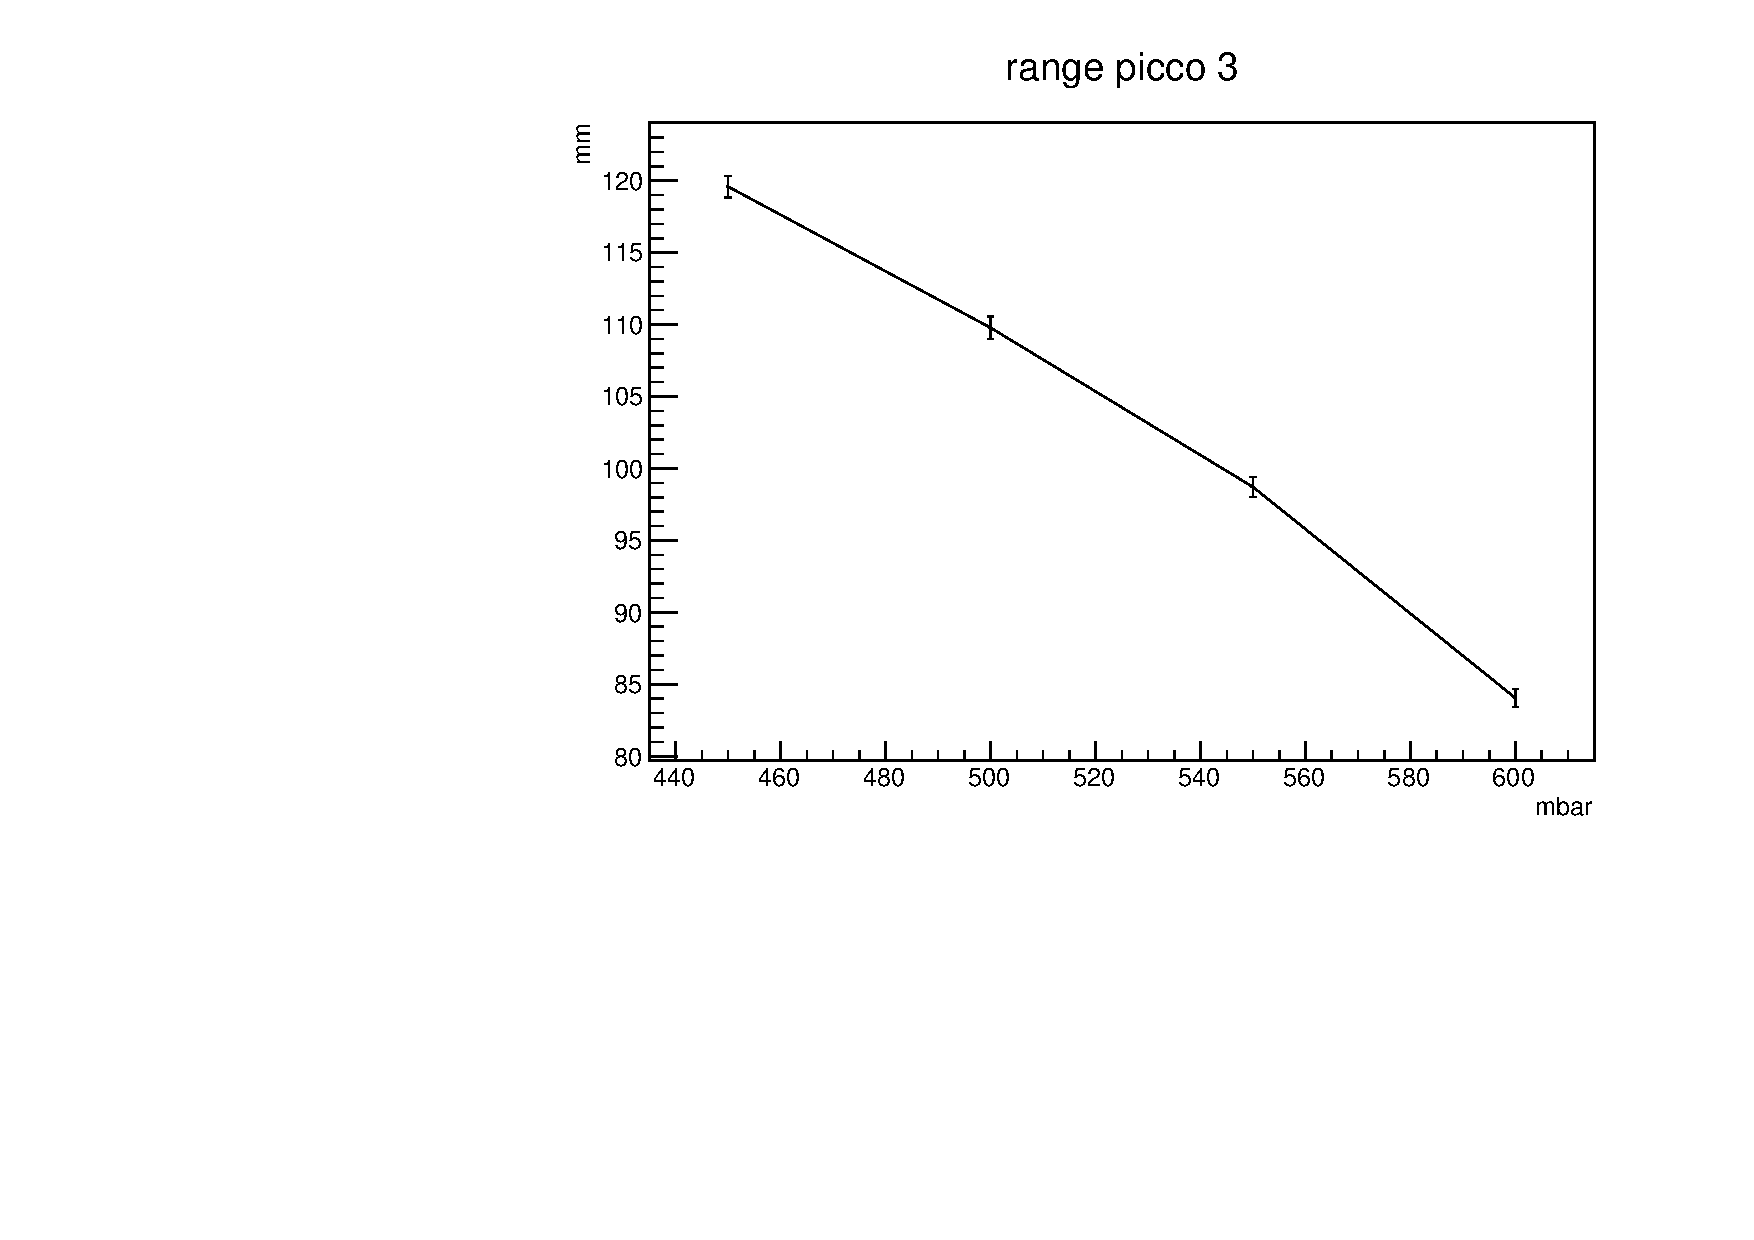
\includegraphics{../grafici/risultati/rangepicco3.pdf}
 }%
 \caption{Grafico Range ($mm$) su Pressione ($mb$) picco 3} 
 \label{gr:rangepicco3.tex} 
\end{grafico}











Infine, ad alte pressioni, è stato verificato che il range spaziale fosse inversamente proporzionale alla pressione.

\begin{grafico}
 \centering
 \resizebox{\textwidth}{!}{%
 \begin{tikzpicture}
\pgfdeclareplotmark{cross} {
\pgfpathmoveto{\pgfpoint{-0.3\pgfplotmarksize}{\pgfplotmarksize}}
\pgfpathlineto{\pgfpoint{+0.3\pgfplotmarksize}{\pgfplotmarksize}}
\pgfpathlineto{\pgfpoint{+0.3\pgfplotmarksize}{0.3\pgfplotmarksize}}
\pgfpathlineto{\pgfpoint{+1\pgfplotmarksize}{0.3\pgfplotmarksize}}
\pgfpathlineto{\pgfpoint{+1\pgfplotmarksize}{-0.3\pgfplotmarksize}}
\pgfpathlineto{\pgfpoint{+0.3\pgfplotmarksize}{-0.3\pgfplotmarksize}}
\pgfpathlineto{\pgfpoint{+0.3\pgfplotmarksize}{-1.\pgfplotmarksize}}
\pgfpathlineto{\pgfpoint{-0.3\pgfplotmarksize}{-1.\pgfplotmarksize}}
\pgfpathlineto{\pgfpoint{-0.3\pgfplotmarksize}{-0.3\pgfplotmarksize}}
\pgfpathlineto{\pgfpoint{-1.\pgfplotmarksize}{-0.3\pgfplotmarksize}}
\pgfpathlineto{\pgfpoint{-1.\pgfplotmarksize}{0.3\pgfplotmarksize}}
\pgfpathlineto{\pgfpoint{-0.3\pgfplotmarksize}{0.3\pgfplotmarksize}}
\pgfpathclose
\pgfusepathqstroke
}
\pgfdeclareplotmark{cross*} {
\pgfpathmoveto{\pgfpoint{-0.3\pgfplotmarksize}{\pgfplotmarksize}}
\pgfpathlineto{\pgfpoint{+0.3\pgfplotmarksize}{\pgfplotmarksize}}
\pgfpathlineto{\pgfpoint{+0.3\pgfplotmarksize}{0.3\pgfplotmarksize}}
\pgfpathlineto{\pgfpoint{+1\pgfplotmarksize}{0.3\pgfplotmarksize}}
\pgfpathlineto{\pgfpoint{+1\pgfplotmarksize}{-0.3\pgfplotmarksize}}
\pgfpathlineto{\pgfpoint{+0.3\pgfplotmarksize}{-0.3\pgfplotmarksize}}
\pgfpathlineto{\pgfpoint{+0.3\pgfplotmarksize}{-1.\pgfplotmarksize}}
\pgfpathlineto{\pgfpoint{-0.3\pgfplotmarksize}{-1.\pgfplotmarksize}}
\pgfpathlineto{\pgfpoint{-0.3\pgfplotmarksize}{-0.3\pgfplotmarksize}}
\pgfpathlineto{\pgfpoint{-1.\pgfplotmarksize}{-0.3\pgfplotmarksize}}
\pgfpathlineto{\pgfpoint{-1.\pgfplotmarksize}{0.3\pgfplotmarksize}}
\pgfpathlineto{\pgfpoint{-0.3\pgfplotmarksize}{0.3\pgfplotmarksize}}
\pgfpathclose
\pgfusepathqfillstroke
}
\pgfdeclareplotmark{newstar} {
\pgfpathmoveto{\pgfqpoint{0pt}{\pgfplotmarksize}}
\pgfpathlineto{\pgfqpointpolar{44}{0.5\pgfplotmarksize}}
\pgfpathlineto{\pgfqpointpolar{18}{\pgfplotmarksize}}
\pgfpathlineto{\pgfqpointpolar{-20}{0.5\pgfplotmarksize}}
\pgfpathlineto{\pgfqpointpolar{-54}{\pgfplotmarksize}}
\pgfpathlineto{\pgfqpointpolar{-90}{0.5\pgfplotmarksize}}
\pgfpathlineto{\pgfqpointpolar{234}{\pgfplotmarksize}}
\pgfpathlineto{\pgfqpointpolar{198}{0.5\pgfplotmarksize}}
\pgfpathlineto{\pgfqpointpolar{162}{\pgfplotmarksize}}
\pgfpathlineto{\pgfqpointpolar{134}{0.5\pgfplotmarksize}}
\pgfpathclose
\pgfusepathqstroke
}
\pgfdeclareplotmark{newstar*} {
\pgfpathmoveto{\pgfqpoint{0pt}{\pgfplotmarksize}}
\pgfpathlineto{\pgfqpointpolar{44}{0.5\pgfplotmarksize}}
\pgfpathlineto{\pgfqpointpolar{18}{\pgfplotmarksize}}
\pgfpathlineto{\pgfqpointpolar{-20}{0.5\pgfplotmarksize}}
\pgfpathlineto{\pgfqpointpolar{-54}{\pgfplotmarksize}}
\pgfpathlineto{\pgfqpointpolar{-90}{0.5\pgfplotmarksize}}
\pgfpathlineto{\pgfqpointpolar{234}{\pgfplotmarksize}}
\pgfpathlineto{\pgfqpointpolar{198}{0.5\pgfplotmarksize}}
\pgfpathlineto{\pgfqpointpolar{162}{\pgfplotmarksize}}
\pgfpathlineto{\pgfqpointpolar{134}{0.5\pgfplotmarksize}}
\pgfpathclose
\pgfusepathqfillstroke
}
\definecolor{c}{rgb}{1,1,1};
\draw [color=c, fill=c] (0,0) rectangle (20,13.4957);
\draw [color=c, fill=c] (2,1.34957) rectangle (18,12.1461);
\definecolor{c}{rgb}{0,0,0};
\draw [c,line width=0.9] (2,1.34957) -- (2,12.1461) -- (18,12.1461) -- (18,1.34957) -- (2,1.34957);
\definecolor{c}{rgb}{1,1,1};
\draw [color=c, fill=c] (2,1.34957) rectangle (18,12.1461);
\definecolor{c}{rgb}{0,0,0};
\draw [c,line width=0.9] (2,1.34957) -- (2,12.1461) -- (18,12.1461) -- (18,1.34957) -- (2,1.34957);
\draw [c,line width=0.9] (2,1.34957) -- (18,1.34957);
\draw [anchor= east] (18,0.593811) node[scale=1.01821, color=c, rotate=0]{$p\; [mb]$};
\draw [c,line width=0.9] (3.33333,1.67347) -- (3.33333,1.34957);
\draw [c,line width=0.9] (3.86667,1.51152) -- (3.86667,1.34957);
\draw [c,line width=0.9] (4.4,1.51152) -- (4.4,1.34957);
\draw [c,line width=0.9] (4.93333,1.51152) -- (4.93333,1.34957);
\draw [c,line width=0.9] (5.46667,1.51152) -- (5.46667,1.34957);
\draw [c,line width=0.9] (6,1.67347) -- (6,1.34957);
\draw [c,line width=0.9] (6.53333,1.51152) -- (6.53333,1.34957);
\draw [c,line width=0.9] (7.06667,1.51152) -- (7.06667,1.34957);
\draw [c,line width=0.9] (7.6,1.51152) -- (7.6,1.34957);
\draw [c,line width=0.9] (8.13333,1.51152) -- (8.13333,1.34957);
\draw [c,line width=0.9] (8.66667,1.67347) -- (8.66667,1.34957);
\draw [c,line width=0.9] (9.2,1.51152) -- (9.2,1.34957);
\draw [c,line width=0.9] (9.73333,1.51152) -- (9.73333,1.34957);
\draw [c,line width=0.9] (10.2667,1.51152) -- (10.2667,1.34957);
\draw [c,line width=0.9] (10.8,1.51152) -- (10.8,1.34957);
\draw [c,line width=0.9] (11.3333,1.67347) -- (11.3333,1.34957);
\draw [c,line width=0.9] (11.8667,1.51152) -- (11.8667,1.34957);
\draw [c,line width=0.9] (12.4,1.51152) -- (12.4,1.34957);
\draw [c,line width=0.9] (12.9333,1.51152) -- (12.9333,1.34957);
\draw [c,line width=0.9] (13.4667,1.51152) -- (13.4667,1.34957);
\draw [c,line width=0.9] (14,1.67347) -- (14,1.34957);
\draw [c,line width=0.9] (14.5333,1.51152) -- (14.5333,1.34957);
\draw [c,line width=0.9] (15.0667,1.51152) -- (15.0667,1.34957);
\draw [c,line width=0.9] (15.6,1.51152) -- (15.6,1.34957);
\draw [c,line width=0.9] (16.1333,1.51152) -- (16.1333,1.34957);
\draw [c,line width=0.9] (16.6667,1.67347) -- (16.6667,1.34957);
\draw [c,line width=0.9] (3.33333,1.67347) -- (3.33333,1.34957);
\draw [c,line width=0.9] (2.8,1.51152) -- (2.8,1.34957);
\draw [c,line width=0.9] (2.26667,1.51152) -- (2.26667,1.34957);
\draw [c,line width=0.9] (16.6667,1.67347) -- (16.6667,1.34957);
\draw [c,line width=0.9] (17.2,1.51152) -- (17.2,1.34957);
\draw [c,line width=0.9] (17.7333,1.51152) -- (17.7333,1.34957);
\draw [anchor=base] (3.33333,0.904212) node[scale=1.01821, color=c, rotate=0]{400};
\draw [anchor=base] (6,0.904212) node[scale=1.01821, color=c, rotate=0]{450};
\draw [anchor=base] (8.66667,0.904212) node[scale=1.01821, color=c, rotate=0]{500};
\draw [anchor=base] (11.3333,0.904212) node[scale=1.01821, color=c, rotate=0]{550};
\draw [anchor=base] (14,0.904212) node[scale=1.01821, color=c, rotate=0]{600};
\draw [anchor=base] (16.6667,0.904212) node[scale=1.01821, color=c, rotate=0]{650};
\draw [c,line width=0.9] (2,1.34957) -- (2,12.1461);
\draw [anchor= east] (0.88,12.1461) node[scale=1.01821, color=c, rotate=90]{$ R \cdot p \;[mb \cdot m]$};
\draw [c,line width=0.9] (2.48,1.34957) -- (2,1.34957);
\draw [c,line width=0.9] (2.24,1.70946) -- (2,1.70946);
\draw [c,line width=0.9] (2.24,2.06934) -- (2,2.06934);
\draw [c,line width=0.9] (2.24,2.42923) -- (2,2.42923);
\draw [c,line width=0.9] (2.24,2.78911) -- (2,2.78911);
\draw [c,line width=0.9] (2.48,3.149) -- (2,3.149);
\draw [c,line width=0.9] (2.24,3.50888) -- (2,3.50888);
\draw [c,line width=0.9] (2.24,3.86877) -- (2,3.86877);
\draw [c,line width=0.9] (2.24,4.22865) -- (2,4.22865);
\draw [c,line width=0.9] (2.24,4.58854) -- (2,4.58854);
\draw [c,line width=0.9] (2.48,4.94842) -- (2,4.94842);
\draw [c,line width=0.9] (2.24,5.30831) -- (2,5.30831);
\draw [c,line width=0.9] (2.24,5.66819) -- (2,5.66819);
\draw [c,line width=0.9] (2.24,6.02808) -- (2,6.02808);
\draw [c,line width=0.9] (2.24,6.38797) -- (2,6.38797);
\draw [c,line width=0.9] (2.48,6.74785) -- (2,6.74785);
\draw [c,line width=0.9] (2.24,7.10774) -- (2,7.10774);
\draw [c,line width=0.9] (2.24,7.46762) -- (2,7.46762);
\draw [c,line width=0.9] (2.24,7.82751) -- (2,7.82751);
\draw [c,line width=0.9] (2.24,8.18739) -- (2,8.18739);
\draw [c,line width=0.9] (2.48,8.54728) -- (2,8.54728);
\draw [c,line width=0.9] (2.24,8.90716) -- (2,8.90716);
\draw [c,line width=0.9] (2.24,9.26705) -- (2,9.26705);
\draw [c,line width=0.9] (2.24,9.62693) -- (2,9.62693);
\draw [c,line width=0.9] (2.24,9.98682) -- (2,9.98682);
\draw [c,line width=0.9] (2.48,10.3467) -- (2,10.3467);
\draw [c,line width=0.9] (2.24,10.7066) -- (2,10.7066);
\draw [c,line width=0.9] (2.24,11.0665) -- (2,11.0665);
\draw [c,line width=0.9] (2.24,11.4264) -- (2,11.4264);
\draw [c,line width=0.9] (2.24,11.7862) -- (2,11.7862);
\draw [c,line width=0.9] (2.48,12.1461) -- (2,12.1461);
\draw [anchor= east] (1.9,1.34957) node[scale=1.01821, color=c, rotate=0]{0};
\draw [anchor= east] (1.9,3.149) node[scale=1.01821, color=c, rotate=0]{10};
\draw [anchor= east] (1.9,4.94842) node[scale=1.01821, color=c, rotate=0]{20};
\draw [anchor= east] (1.9,6.74785) node[scale=1.01821, color=c, rotate=0]{30};
\draw [anchor= east] (1.9,8.54728) node[scale=1.01821, color=c, rotate=0]{40};
\draw [anchor= east] (1.9,10.3467) node[scale=1.01821, color=c, rotate=0]{50};
\draw [anchor= east] (1.9,12.1461) node[scale=1.01821, color=c, rotate=0]{60};
\draw [c,line width=0.9] (3.33333,9.50584) -- (6,9.70837) -- (8.66667,9.80707) -- (11.3333,9.72685) -- (14,9.17382) -- (16.6667,9.17763);
\foreach \P in {(3.33333,9.50584), (6,9.70837), (8.66667,9.80707), (11.3333,9.72685), (14,9.17382), (16.6667,9.17763)}{\draw[mark options={color=c,fill=c},mark size=2.402402pt,mark=*,mark size=1pt] plot coordinates {\P};}
\draw [c,line width=0.9] (3.33333,9.50584) -- (3.33333,9.5561);
\draw [c,line width=0.9] (3.27603,9.5561) -- (3.39064,9.5561);
\draw [c,line width=0.9] (3.33333,9.50584) -- (3.33333,9.45558);
\draw [c,line width=0.9] (3.27603,9.45558) -- (3.39064,9.45558);
\draw [c,line width=0.9] (6,9.70837) -- (6,9.75992);
\draw [c,line width=0.9] (5.94269,9.75992) -- (6.05731,9.75992);
\draw [c,line width=0.9] (6,9.70837) -- (6,9.65682);
\draw [c,line width=0.9] (5.94269,9.65682) -- (6.05731,9.65682);
\draw [c,line width=0.9] (8.66667,9.80707) -- (8.66667,9.85928);
\draw [c,line width=0.9] (8.60936,9.85928) -- (8.72397,9.85928);
\draw [c,line width=0.9] (8.66667,9.80707) -- (8.66667,9.75485);
\draw [c,line width=0.9] (8.60936,9.75485) -- (8.72397,9.75485);
\draw [c,line width=0.9] (11.3333,9.72685) -- (11.3333,9.77847);
\draw [c,line width=0.9] (11.276,9.77847) -- (11.3906,9.77847);
\draw [c,line width=0.9] (11.3333,9.72685) -- (11.3333,9.67522);
\draw [c,line width=0.9] (11.276,9.67522) -- (11.3906,9.67522);
\draw [c,line width=0.9] (14,9.17382) -- (14,9.22195);
\draw [c,line width=0.9] (13.9427,9.22195) -- (14.0573,9.22195);
\draw [c,line width=0.9] (14,9.17382) -- (14,9.12569);
\draw [c,line width=0.9] (13.9427,9.12569) -- (14.0573,9.12569);
\draw [c,line width=0.9] (16.6667,9.17763) -- (16.6667,9.22659);
\draw [c,line width=0.9] (16.6094,9.22659) -- (16.724,9.22659);
\draw [c,line width=0.9] (16.6667,9.17763) -- (16.6667,9.12867);
\draw [c,line width=0.9] (16.6094,9.12867) -- (16.724,9.12867);
\draw (9.67049,13.0156) node[scale=1.52731, color=c, rotate=0]{$R \cdot p$};
\end{tikzpicture}

 }%
 \caption{Grafico Range ($m \cdot b$) su Pressione ($mb$)} 
 \label{gr:rp1.tex} 
\end{grafico}


\begin{grafico}
 \centering
 \resizebox{\textwidth}{!}{%
 \begin{tikzpicture}
\pgfdeclareplotmark{cross} {
\pgfpathmoveto{\pgfpoint{-0.3\pgfplotmarksize}{\pgfplotmarksize}}
\pgfpathlineto{\pgfpoint{+0.3\pgfplotmarksize}{\pgfplotmarksize}}
\pgfpathlineto{\pgfpoint{+0.3\pgfplotmarksize}{0.3\pgfplotmarksize}}
\pgfpathlineto{\pgfpoint{+1\pgfplotmarksize}{0.3\pgfplotmarksize}}
\pgfpathlineto{\pgfpoint{+1\pgfplotmarksize}{-0.3\pgfplotmarksize}}
\pgfpathlineto{\pgfpoint{+0.3\pgfplotmarksize}{-0.3\pgfplotmarksize}}
\pgfpathlineto{\pgfpoint{+0.3\pgfplotmarksize}{-1.\pgfplotmarksize}}
\pgfpathlineto{\pgfpoint{-0.3\pgfplotmarksize}{-1.\pgfplotmarksize}}
\pgfpathlineto{\pgfpoint{-0.3\pgfplotmarksize}{-0.3\pgfplotmarksize}}
\pgfpathlineto{\pgfpoint{-1.\pgfplotmarksize}{-0.3\pgfplotmarksize}}
\pgfpathlineto{\pgfpoint{-1.\pgfplotmarksize}{0.3\pgfplotmarksize}}
\pgfpathlineto{\pgfpoint{-0.3\pgfplotmarksize}{0.3\pgfplotmarksize}}
\pgfpathclose
\pgfusepathqstroke
}
\pgfdeclareplotmark{cross*} {
\pgfpathmoveto{\pgfpoint{-0.3\pgfplotmarksize}{\pgfplotmarksize}}
\pgfpathlineto{\pgfpoint{+0.3\pgfplotmarksize}{\pgfplotmarksize}}
\pgfpathlineto{\pgfpoint{+0.3\pgfplotmarksize}{0.3\pgfplotmarksize}}
\pgfpathlineto{\pgfpoint{+1\pgfplotmarksize}{0.3\pgfplotmarksize}}
\pgfpathlineto{\pgfpoint{+1\pgfplotmarksize}{-0.3\pgfplotmarksize}}
\pgfpathlineto{\pgfpoint{+0.3\pgfplotmarksize}{-0.3\pgfplotmarksize}}
\pgfpathlineto{\pgfpoint{+0.3\pgfplotmarksize}{-1.\pgfplotmarksize}}
\pgfpathlineto{\pgfpoint{-0.3\pgfplotmarksize}{-1.\pgfplotmarksize}}
\pgfpathlineto{\pgfpoint{-0.3\pgfplotmarksize}{-0.3\pgfplotmarksize}}
\pgfpathlineto{\pgfpoint{-1.\pgfplotmarksize}{-0.3\pgfplotmarksize}}
\pgfpathlineto{\pgfpoint{-1.\pgfplotmarksize}{0.3\pgfplotmarksize}}
\pgfpathlineto{\pgfpoint{-0.3\pgfplotmarksize}{0.3\pgfplotmarksize}}
\pgfpathclose
\pgfusepathqfillstroke
}
\pgfdeclareplotmark{newstar} {
\pgfpathmoveto{\pgfqpoint{0pt}{\pgfplotmarksize}}
\pgfpathlineto{\pgfqpointpolar{44}{0.5\pgfplotmarksize}}
\pgfpathlineto{\pgfqpointpolar{18}{\pgfplotmarksize}}
\pgfpathlineto{\pgfqpointpolar{-20}{0.5\pgfplotmarksize}}
\pgfpathlineto{\pgfqpointpolar{-54}{\pgfplotmarksize}}
\pgfpathlineto{\pgfqpointpolar{-90}{0.5\pgfplotmarksize}}
\pgfpathlineto{\pgfqpointpolar{234}{\pgfplotmarksize}}
\pgfpathlineto{\pgfqpointpolar{198}{0.5\pgfplotmarksize}}
\pgfpathlineto{\pgfqpointpolar{162}{\pgfplotmarksize}}
\pgfpathlineto{\pgfqpointpolar{134}{0.5\pgfplotmarksize}}
\pgfpathclose
\pgfusepathqstroke
}
\pgfdeclareplotmark{newstar*} {
\pgfpathmoveto{\pgfqpoint{0pt}{\pgfplotmarksize}}
\pgfpathlineto{\pgfqpointpolar{44}{0.5\pgfplotmarksize}}
\pgfpathlineto{\pgfqpointpolar{18}{\pgfplotmarksize}}
\pgfpathlineto{\pgfqpointpolar{-20}{0.5\pgfplotmarksize}}
\pgfpathlineto{\pgfqpointpolar{-54}{\pgfplotmarksize}}
\pgfpathlineto{\pgfqpointpolar{-90}{0.5\pgfplotmarksize}}
\pgfpathlineto{\pgfqpointpolar{234}{\pgfplotmarksize}}
\pgfpathlineto{\pgfqpointpolar{198}{0.5\pgfplotmarksize}}
\pgfpathlineto{\pgfqpointpolar{162}{\pgfplotmarksize}}
\pgfpathlineto{\pgfqpointpolar{134}{0.5\pgfplotmarksize}}
\pgfpathclose
\pgfusepathqfillstroke
}
\definecolor{c}{rgb}{1,1,1};
\draw [color=c, fill=c] (0,0) rectangle (20,13.4957);
\draw [color=c, fill=c] (2,1.34957) rectangle (18,12.1461);
\definecolor{c}{rgb}{0,0,0};
\draw [c,line width=0.9] (2,1.34957) -- (2,12.1461) -- (18,12.1461) -- (18,1.34957) -- (2,1.34957);
\definecolor{c}{rgb}{1,1,1};
\draw [color=c, fill=c] (2,1.34957) rectangle (18,12.1461);
\definecolor{c}{rgb}{0,0,0};
\draw [c,line width=0.9] (2,1.34957) -- (2,12.1461) -- (18,12.1461) -- (18,1.34957) -- (2,1.34957);
\draw [c,line width=0.9] (2,1.34957) -- (18,1.34957);
\draw [anchor= east] (18,0.593811) node[scale=1.01821, color=c, rotate=0]{$p \;[mb]$};
\draw [c,line width=0.9] (3.33333,1.67347) -- (3.33333,1.34957);
\draw [c,line width=0.9] (4,1.51152) -- (4,1.34957);
\draw [c,line width=0.9] (4.66667,1.51152) -- (4.66667,1.34957);
\draw [c,line width=0.9] (5.33333,1.51152) -- (5.33333,1.34957);
\draw [c,line width=0.9] (6,1.51152) -- (6,1.34957);
\draw [c,line width=0.9] (6.66667,1.67347) -- (6.66667,1.34957);
\draw [c,line width=0.9] (7.33333,1.51152) -- (7.33333,1.34957);
\draw [c,line width=0.9] (8,1.51152) -- (8,1.34957);
\draw [c,line width=0.9] (8.66667,1.51152) -- (8.66667,1.34957);
\draw [c,line width=0.9] (9.33333,1.51152) -- (9.33333,1.34957);
\draw [c,line width=0.9] (10,1.67347) -- (10,1.34957);
\draw [c,line width=0.9] (10.6667,1.51152) -- (10.6667,1.34957);
\draw [c,line width=0.9] (11.3333,1.51152) -- (11.3333,1.34957);
\draw [c,line width=0.9] (12,1.51152) -- (12,1.34957);
\draw [c,line width=0.9] (12.6667,1.51152) -- (12.6667,1.34957);
\draw [c,line width=0.9] (13.3333,1.67347) -- (13.3333,1.34957);
\draw [c,line width=0.9] (14,1.51152) -- (14,1.34957);
\draw [c,line width=0.9] (14.6667,1.51152) -- (14.6667,1.34957);
\draw [c,line width=0.9] (15.3333,1.51152) -- (15.3333,1.34957);
\draw [c,line width=0.9] (16,1.51152) -- (16,1.34957);
\draw [c,line width=0.9] (16.6667,1.67347) -- (16.6667,1.34957);
\draw [c,line width=0.9] (3.33333,1.67347) -- (3.33333,1.34957);
\draw [c,line width=0.9] (2.66667,1.51152) -- (2.66667,1.34957);
\draw [c,line width=0.9] (2,1.51152) -- (2,1.34957);
\draw [c,line width=0.9] (16.6667,1.67347) -- (16.6667,1.34957);
\draw [c,line width=0.9] (17.3333,1.51152) -- (17.3333,1.34957);
\draw [anchor=base] (3.33333,0.904212) node[scale=1.01821, color=c, rotate=0]{400};
\draw [anchor=base] (6.66667,0.904212) node[scale=1.01821, color=c, rotate=0]{450};
\draw [anchor=base] (10,0.904212) node[scale=1.01821, color=c, rotate=0]{500};
\draw [anchor=base] (13.3333,0.904212) node[scale=1.01821, color=c, rotate=0]{550};
\draw [anchor=base] (16.6667,0.904212) node[scale=1.01821, color=c, rotate=0]{600};
\draw [c,line width=0.9] (2,1.34957) -- (2,12.1461);
\draw [anchor= east] (0.88,12.1461) node[scale=1.01821, color=c, rotate=90]{$R \cdot p \;[mb \cdot m]$};
\draw [c,line width=0.9] (2.48,1.34957) -- (2,1.34957);
\draw [c,line width=0.9] (2.24,1.68177) -- (2,1.68177);
\draw [c,line width=0.9] (2.24,2.01397) -- (2,2.01397);
\draw [c,line width=0.9] (2.24,2.34618) -- (2,2.34618);
\draw [c,line width=0.9] (2.24,2.67838) -- (2,2.67838);
\draw [c,line width=0.9] (2.48,3.01058) -- (2,3.01058);
\draw [c,line width=0.9] (2.24,3.34278) -- (2,3.34278);
\draw [c,line width=0.9] (2.24,3.67498) -- (2,3.67498);
\draw [c,line width=0.9] (2.24,4.00719) -- (2,4.00719);
\draw [c,line width=0.9] (2.24,4.33939) -- (2,4.33939);
\draw [c,line width=0.9] (2.48,4.67159) -- (2,4.67159);
\draw [c,line width=0.9] (2.24,5.00379) -- (2,5.00379);
\draw [c,line width=0.9] (2.24,5.33599) -- (2,5.33599);
\draw [c,line width=0.9] (2.24,5.66819) -- (2,5.66819);
\draw [c,line width=0.9] (2.24,6.0004) -- (2,6.0004);
\draw [c,line width=0.9] (2.48,6.3326) -- (2,6.3326);
\draw [c,line width=0.9] (2.24,6.6648) -- (2,6.6648);
\draw [c,line width=0.9] (2.24,6.997) -- (2,6.997);
\draw [c,line width=0.9] (2.24,7.3292) -- (2,7.3292);
\draw [c,line width=0.9] (2.24,7.66141) -- (2,7.66141);
\draw [c,line width=0.9] (2.48,7.99361) -- (2,7.99361);
\draw [c,line width=0.9] (2.24,8.32581) -- (2,8.32581);
\draw [c,line width=0.9] (2.24,8.65801) -- (2,8.65801);
\draw [c,line width=0.9] (2.24,8.99021) -- (2,8.99021);
\draw [c,line width=0.9] (2.24,9.32242) -- (2,9.32242);
\draw [c,line width=0.9] (2.48,9.65462) -- (2,9.65462);
\draw [c,line width=0.9] (2.24,9.98682) -- (2,9.98682);
\draw [c,line width=0.9] (2.24,10.319) -- (2,10.319);
\draw [c,line width=0.9] (2.24,10.6512) -- (2,10.6512);
\draw [c,line width=0.9] (2.24,10.9834) -- (2,10.9834);
\draw [c,line width=0.9] (2.48,11.3156) -- (2,11.3156);
\draw [c,line width=0.9] (2.48,11.3156) -- (2,11.3156);
\draw [c,line width=0.9] (2.24,11.6478) -- (2,11.6478);
\draw [c,line width=0.9] (2.24,11.98) -- (2,11.98);
\draw [anchor= east] (1.9,1.34957) node[scale=1.01821, color=c, rotate=0]{0};
\draw [anchor= east] (1.9,3.01058) node[scale=1.01821, color=c, rotate=0]{10};
\draw [anchor= east] (1.9,4.67159) node[scale=1.01821, color=c, rotate=0]{20};
\draw [anchor= east] (1.9,6.3326) node[scale=1.01821, color=c, rotate=0]{30};
\draw [anchor= east] (1.9,7.99361) node[scale=1.01821, color=c, rotate=0]{40};
\draw [anchor= east] (1.9,9.65462) node[scale=1.01821, color=c, rotate=0]{50};
\draw [anchor= east] (1.9,11.3156) node[scale=1.01821, color=c, rotate=0]{60};
\draw [c,line width=0.9] (3.33333,9.58562) -- (6.66667,9.70258) -- (10,9.8347) -- (13.3333,9.7302) -- (16.6667,9.15026);
\foreach \P in {(3.33333,9.58562), (6.66667,9.70258), (10,9.8347), (13.3333,9.7302), (16.6667,9.15026)}{\draw[mark options={color=c,fill=c},mark size=2.402402pt,mark=*,mark size=1pt] plot coordinates {\P};}
\draw [c,line width=0.9] (3.33333,9.58562) -- (3.33333,9.63656);
\draw [c,line width=0.9] (3.27603,9.63656) -- (3.39064,9.63656);
\draw [c,line width=0.9] (3.33333,9.58562) -- (3.33333,9.53467);
\draw [c,line width=0.9] (3.27603,9.53467) -- (3.39064,9.53467);
\draw [c,line width=0.9] (6.66667,9.70258) -- (6.66667,9.75419);
\draw [c,line width=0.9] (6.60936,9.75419) -- (6.72397,9.75419);
\draw [c,line width=0.9] (6.66667,9.70258) -- (6.66667,9.65097);
\draw [c,line width=0.9] (6.60936,9.65097) -- (6.72397,9.65097);
\draw [c,line width=0.9] (10,9.8347) -- (10,9.8872);
\draw [c,line width=0.9] (9.94269,9.8872) -- (10.0573,9.8872);
\draw [c,line width=0.9] (10,9.8347) -- (10,9.78221);
\draw [c,line width=0.9] (9.94269,9.78221) -- (10.0573,9.78221);
\draw [c,line width=0.9] (13.3333,9.7302) -- (13.3333,9.78181);
\draw [c,line width=0.9] (13.276,9.78181) -- (13.3906,9.78181);
\draw [c,line width=0.9] (13.3333,9.7302) -- (13.3333,9.67859);
\draw [c,line width=0.9] (13.276,9.67859) -- (13.3906,9.67859);
\draw [c,line width=0.9] (16.6667,9.15026) -- (16.6667,9.19837);
\draw [c,line width=0.9] (16.6094,9.19837) -- (16.724,9.19837);
\draw [c,line width=0.9] (16.6667,9.15026) -- (16.6667,9.10216);
\draw [c,line width=0.9] (16.6094,9.10216) -- (16.724,9.10216);
\draw (9.67049,13.0156) node[scale=1.52731, color=c, rotate=0]{$R \cdot p$};
\end{tikzpicture}

 }%
 \caption{Grafico Range ($m \cdot b$) su Pressione ($mb$)} 
 \label{gr:rp2.tex} 
\end{grafico}


\begin{grafico}
 \centering
 \resizebox{\textwidth}{!}{%
 \begin{tikzpicture}
\pgfdeclareplotmark{cross} {
\pgfpathmoveto{\pgfpoint{-0.3\pgfplotmarksize}{\pgfplotmarksize}}
\pgfpathlineto{\pgfpoint{+0.3\pgfplotmarksize}{\pgfplotmarksize}}
\pgfpathlineto{\pgfpoint{+0.3\pgfplotmarksize}{0.3\pgfplotmarksize}}
\pgfpathlineto{\pgfpoint{+1\pgfplotmarksize}{0.3\pgfplotmarksize}}
\pgfpathlineto{\pgfpoint{+1\pgfplotmarksize}{-0.3\pgfplotmarksize}}
\pgfpathlineto{\pgfpoint{+0.3\pgfplotmarksize}{-0.3\pgfplotmarksize}}
\pgfpathlineto{\pgfpoint{+0.3\pgfplotmarksize}{-1.\pgfplotmarksize}}
\pgfpathlineto{\pgfpoint{-0.3\pgfplotmarksize}{-1.\pgfplotmarksize}}
\pgfpathlineto{\pgfpoint{-0.3\pgfplotmarksize}{-0.3\pgfplotmarksize}}
\pgfpathlineto{\pgfpoint{-1.\pgfplotmarksize}{-0.3\pgfplotmarksize}}
\pgfpathlineto{\pgfpoint{-1.\pgfplotmarksize}{0.3\pgfplotmarksize}}
\pgfpathlineto{\pgfpoint{-0.3\pgfplotmarksize}{0.3\pgfplotmarksize}}
\pgfpathclose
\pgfusepathqstroke
}
\pgfdeclareplotmark{cross*} {
\pgfpathmoveto{\pgfpoint{-0.3\pgfplotmarksize}{\pgfplotmarksize}}
\pgfpathlineto{\pgfpoint{+0.3\pgfplotmarksize}{\pgfplotmarksize}}
\pgfpathlineto{\pgfpoint{+0.3\pgfplotmarksize}{0.3\pgfplotmarksize}}
\pgfpathlineto{\pgfpoint{+1\pgfplotmarksize}{0.3\pgfplotmarksize}}
\pgfpathlineto{\pgfpoint{+1\pgfplotmarksize}{-0.3\pgfplotmarksize}}
\pgfpathlineto{\pgfpoint{+0.3\pgfplotmarksize}{-0.3\pgfplotmarksize}}
\pgfpathlineto{\pgfpoint{+0.3\pgfplotmarksize}{-1.\pgfplotmarksize}}
\pgfpathlineto{\pgfpoint{-0.3\pgfplotmarksize}{-1.\pgfplotmarksize}}
\pgfpathlineto{\pgfpoint{-0.3\pgfplotmarksize}{-0.3\pgfplotmarksize}}
\pgfpathlineto{\pgfpoint{-1.\pgfplotmarksize}{-0.3\pgfplotmarksize}}
\pgfpathlineto{\pgfpoint{-1.\pgfplotmarksize}{0.3\pgfplotmarksize}}
\pgfpathlineto{\pgfpoint{-0.3\pgfplotmarksize}{0.3\pgfplotmarksize}}
\pgfpathclose
\pgfusepathqfillstroke
}
\pgfdeclareplotmark{newstar} {
\pgfpathmoveto{\pgfqpoint{0pt}{\pgfplotmarksize}}
\pgfpathlineto{\pgfqpointpolar{44}{0.5\pgfplotmarksize}}
\pgfpathlineto{\pgfqpointpolar{18}{\pgfplotmarksize}}
\pgfpathlineto{\pgfqpointpolar{-20}{0.5\pgfplotmarksize}}
\pgfpathlineto{\pgfqpointpolar{-54}{\pgfplotmarksize}}
\pgfpathlineto{\pgfqpointpolar{-90}{0.5\pgfplotmarksize}}
\pgfpathlineto{\pgfqpointpolar{234}{\pgfplotmarksize}}
\pgfpathlineto{\pgfqpointpolar{198}{0.5\pgfplotmarksize}}
\pgfpathlineto{\pgfqpointpolar{162}{\pgfplotmarksize}}
\pgfpathlineto{\pgfqpointpolar{134}{0.5\pgfplotmarksize}}
\pgfpathclose
\pgfusepathqstroke
}
\pgfdeclareplotmark{newstar*} {
\pgfpathmoveto{\pgfqpoint{0pt}{\pgfplotmarksize}}
\pgfpathlineto{\pgfqpointpolar{44}{0.5\pgfplotmarksize}}
\pgfpathlineto{\pgfqpointpolar{18}{\pgfplotmarksize}}
\pgfpathlineto{\pgfqpointpolar{-20}{0.5\pgfplotmarksize}}
\pgfpathlineto{\pgfqpointpolar{-54}{\pgfplotmarksize}}
\pgfpathlineto{\pgfqpointpolar{-90}{0.5\pgfplotmarksize}}
\pgfpathlineto{\pgfqpointpolar{234}{\pgfplotmarksize}}
\pgfpathlineto{\pgfqpointpolar{198}{0.5\pgfplotmarksize}}
\pgfpathlineto{\pgfqpointpolar{162}{\pgfplotmarksize}}
\pgfpathlineto{\pgfqpointpolar{134}{0.5\pgfplotmarksize}}
\pgfpathclose
\pgfusepathqfillstroke
}
\definecolor{c}{rgb}{1,1,1};
\draw [color=c, fill=c] (0,0) rectangle (20,13.4957);
\draw [color=c, fill=c] (2,1.34957) rectangle (18,12.1461);
\definecolor{c}{rgb}{0,0,0};
\draw [c,line width=0.9] (2,1.34957) -- (2,12.1461) -- (18,12.1461) -- (18,1.34957) -- (2,1.34957);
\definecolor{c}{rgb}{1,1,1};
\draw [color=c, fill=c] (2,1.34957) rectangle (18,12.1461);
\definecolor{c}{rgb}{0,0,0};
\draw [c,line width=0.9] (2,1.34957) -- (2,12.1461) -- (18,12.1461) -- (18,1.34957) -- (2,1.34957);
\draw [c,line width=0.9] (2,1.34957) -- (18,1.34957);
\draw [anchor= east] (18,0.593811) node[scale=1.01821, color=c, rotate=0]{$p\;[mb]$};
\draw [c,line width=0.9] (2.44444,1.67347) -- (2.44444,1.34957);
\draw [c,line width=0.9] (2.88889,1.51152) -- (2.88889,1.34957);
\draw [c,line width=0.9] (3.33333,1.51152) -- (3.33333,1.34957);
\draw [c,line width=0.9] (3.77778,1.51152) -- (3.77778,1.34957);
\draw [c,line width=0.9] (4.22222,1.67347) -- (4.22222,1.34957);
\draw [c,line width=0.9] (4.66667,1.51152) -- (4.66667,1.34957);
\draw [c,line width=0.9] (5.11111,1.51152) -- (5.11111,1.34957);
\draw [c,line width=0.9] (5.55556,1.51152) -- (5.55556,1.34957);
\draw [c,line width=0.9] (6,1.67347) -- (6,1.34957);
\draw [c,line width=0.9] (6.44444,1.51152) -- (6.44444,1.34957);
\draw [c,line width=0.9] (6.88889,1.51152) -- (6.88889,1.34957);
\draw [c,line width=0.9] (7.33333,1.51152) -- (7.33333,1.34957);
\draw [c,line width=0.9] (7.77778,1.67347) -- (7.77778,1.34957);
\draw [c,line width=0.9] (8.22222,1.51152) -- (8.22222,1.34957);
\draw [c,line width=0.9] (8.66667,1.51152) -- (8.66667,1.34957);
\draw [c,line width=0.9] (9.11111,1.51152) -- (9.11111,1.34957);
\draw [c,line width=0.9] (9.55556,1.67347) -- (9.55556,1.34957);
\draw [c,line width=0.9] (10,1.51152) -- (10,1.34957);
\draw [c,line width=0.9] (10.4444,1.51152) -- (10.4444,1.34957);
\draw [c,line width=0.9] (10.8889,1.51152) -- (10.8889,1.34957);
\draw [c,line width=0.9] (11.3333,1.67347) -- (11.3333,1.34957);
\draw [c,line width=0.9] (11.7778,1.51152) -- (11.7778,1.34957);
\draw [c,line width=0.9] (12.2222,1.51152) -- (12.2222,1.34957);
\draw [c,line width=0.9] (12.6667,1.51152) -- (12.6667,1.34957);
\draw [c,line width=0.9] (13.1111,1.67347) -- (13.1111,1.34957);
\draw [c,line width=0.9] (13.5556,1.51152) -- (13.5556,1.34957);
\draw [c,line width=0.9] (14,1.51152) -- (14,1.34957);
\draw [c,line width=0.9] (14.4444,1.51152) -- (14.4444,1.34957);
\draw [c,line width=0.9] (14.8889,1.67347) -- (14.8889,1.34957);
\draw [c,line width=0.9] (15.3333,1.51152) -- (15.3333,1.34957);
\draw [c,line width=0.9] (15.7778,1.51152) -- (15.7778,1.34957);
\draw [c,line width=0.9] (16.2222,1.51152) -- (16.2222,1.34957);
\draw [c,line width=0.9] (16.6667,1.67347) -- (16.6667,1.34957);
\draw [c,line width=0.9] (2.44444,1.67347) -- (2.44444,1.34957);
\draw [c,line width=0.9] (2,1.51152) -- (2,1.34957);
\draw [c,line width=0.9] (16.6667,1.67347) -- (16.6667,1.34957);
\draw [c,line width=0.9] (17.1111,1.51152) -- (17.1111,1.34957);
\draw [c,line width=0.9] (17.5556,1.51152) -- (17.5556,1.34957);
\draw [anchor=base] (2.44444,0.904212) node[scale=1.01821, color=c, rotate=0]{440};
\draw [anchor=base] (4.22222,0.904212) node[scale=1.01821, color=c, rotate=0]{460};
\draw [anchor=base] (6,0.904212) node[scale=1.01821, color=c, rotate=0]{480};
\draw [anchor=base] (7.77778,0.904212) node[scale=1.01821, color=c, rotate=0]{500};
\draw [anchor=base] (9.55556,0.904212) node[scale=1.01821, color=c, rotate=0]{520};
\draw [anchor=base] (11.3333,0.904212) node[scale=1.01821, color=c, rotate=0]{540};
\draw [anchor=base] (13.1111,0.904212) node[scale=1.01821, color=c, rotate=0]{560};
\draw [anchor=base] (14.8889,0.904212) node[scale=1.01821, color=c, rotate=0]{580};
\draw [anchor=base] (16.6667,0.904212) node[scale=1.01821, color=c, rotate=0]{600};
\draw [c,line width=0.9] (2,1.34957) -- (2,12.1461);
\draw [anchor= east] (0.88,12.1461) node[scale=1.01821, color=c, rotate=90]{$R\cdot p \; [ mb \cdot m]$};
\draw [c,line width=0.9] (2.48,1.34957) -- (2,1.34957);
\draw [c,line width=0.9] (2.24,1.65804) -- (2,1.65804);
\draw [c,line width=0.9] (2.24,1.96652) -- (2,1.96652);
\draw [c,line width=0.9] (2.24,2.27499) -- (2,2.27499);
\draw [c,line width=0.9] (2.24,2.58346) -- (2,2.58346);
\draw [c,line width=0.9] (2.48,2.89194) -- (2,2.89194);
\draw [c,line width=0.9] (2.24,3.20041) -- (2,3.20041);
\draw [c,line width=0.9] (2.24,3.50888) -- (2,3.50888);
\draw [c,line width=0.9] (2.24,3.81736) -- (2,3.81736);
\draw [c,line width=0.9] (2.24,4.12583) -- (2,4.12583);
\draw [c,line width=0.9] (2.48,4.4343) -- (2,4.4343);
\draw [c,line width=0.9] (2.24,4.74278) -- (2,4.74278);
\draw [c,line width=0.9] (2.24,5.05125) -- (2,5.05125);
\draw [c,line width=0.9] (2.24,5.35972) -- (2,5.35972);
\draw [c,line width=0.9] (2.24,5.66819) -- (2,5.66819);
\draw [c,line width=0.9] (2.48,5.97667) -- (2,5.97667);
\draw [c,line width=0.9] (2.24,6.28514) -- (2,6.28514);
\draw [c,line width=0.9] (2.24,6.59361) -- (2,6.59361);
\draw [c,line width=0.9] (2.24,6.90209) -- (2,6.90209);
\draw [c,line width=0.9] (2.24,7.21056) -- (2,7.21056);
\draw [c,line width=0.9] (2.48,7.51903) -- (2,7.51903);
\draw [c,line width=0.9] (2.24,7.82751) -- (2,7.82751);
\draw [c,line width=0.9] (2.24,8.13598) -- (2,8.13598);
\draw [c,line width=0.9] (2.24,8.44445) -- (2,8.44445);
\draw [c,line width=0.9] (2.24,8.75293) -- (2,8.75293);
\draw [c,line width=0.9] (2.48,9.0614) -- (2,9.0614);
\draw [c,line width=0.9] (2.24,9.36987) -- (2,9.36987);
\draw [c,line width=0.9] (2.24,9.67835) -- (2,9.67835);
\draw [c,line width=0.9] (2.24,9.98682) -- (2,9.98682);
\draw [c,line width=0.9] (2.24,10.2953) -- (2,10.2953);
\draw [c,line width=0.9] (2.48,10.6038) -- (2,10.6038);
\draw [c,line width=0.9] (2.24,10.9122) -- (2,10.9122);
\draw [c,line width=0.9] (2.24,11.2207) -- (2,11.2207);
\draw [c,line width=0.9] (2.24,11.5292) -- (2,11.5292);
\draw [c,line width=0.9] (2.24,11.8377) -- (2,11.8377);
\draw [c,line width=0.9] (2.48,12.1461) -- (2,12.1461);
\draw [anchor= east] (1.9,1.34957) node[scale=1.01821, color=c, rotate=0]{0};
\draw [anchor= east] (1.9,2.89194) node[scale=1.01821, color=c, rotate=0]{10};
\draw [anchor= east] (1.9,4.4343) node[scale=1.01821, color=c, rotate=0]{20};
\draw [anchor= east] (1.9,5.97667) node[scale=1.01821, color=c, rotate=0]{30};
\draw [anchor= east] (1.9,7.51903) node[scale=1.01821, color=c, rotate=0]{40};
\draw [anchor= east] (1.9,9.0614) node[scale=1.01821, color=c, rotate=0]{50};
\draw [anchor= east] (1.9,10.6038) node[scale=1.01821, color=c, rotate=0]{60};
\draw [anchor= east] (1.9,12.1461) node[scale=1.01821, color=c, rotate=0]{70};
\draw [c,line width=0.9] (3.33333,9.6501) -- (7.77778,9.81565) -- (12.2222,9.72339) -- (16.6667,9.12706);
\foreach \P in {(3.33333,9.6501), (7.77778,9.81565), (12.2222,9.72339), (16.6667,9.12706)}{\draw[mark options={color=c,fill=c},mark size=2.402402pt,mark=*,mark size=1pt] plot coordinates {\P};}
\draw [c,line width=0.9] (3.33333,9.6501) -- (3.33333,9.70189);
\draw [c,line width=0.9] (3.27603,9.70189) -- (3.39064,9.70189);
\draw [c,line width=0.9] (3.33333,9.6501) -- (3.33333,9.59832);
\draw [c,line width=0.9] (3.27603,9.59832) -- (3.39064,9.59832);
\draw [c,line width=0.9] (7.77778,9.81565) -- (7.77778,9.87473);
\draw [c,line width=0.9] (7.72047,9.87473) -- (7.83508,9.87473);
\draw [c,line width=0.9] (7.77778,9.81565) -- (7.77778,9.75658);
\draw [c,line width=0.9] (7.72047,9.75658) -- (7.83508,9.75658);
\draw [c,line width=0.9] (12.2222,9.72339) -- (12.2222,9.78207);
\draw [c,line width=0.9] (12.1649,9.78207) -- (12.2795,9.78207);
\draw [c,line width=0.9] (12.2222,9.72339) -- (12.2222,9.66471);
\draw [c,line width=0.9] (12.1649,9.66471) -- (12.2795,9.66471);
\draw [c,line width=0.9] (16.6667,9.12706) -- (16.6667,9.18552);
\draw [c,line width=0.9] (16.6094,9.18552) -- (16.724,9.18552);
\draw [c,line width=0.9] (16.6667,9.12706) -- (16.6667,9.06859);
\draw [c,line width=0.9] (16.6094,9.06859) -- (16.724,9.06859);
\draw (9.67049,13.0156) node[scale=1.52731, color=c, rotate=0]{$R\cdot p$};
\end{tikzpicture}

 }%
 \caption{Grafico Range ($m \cdot b$) su Pressione ($mb$)} 
 \label{gr:rp3.tex} 
\end{grafico}